\documentclass{standalone}
\usepackage{tikz}
\begin{document}
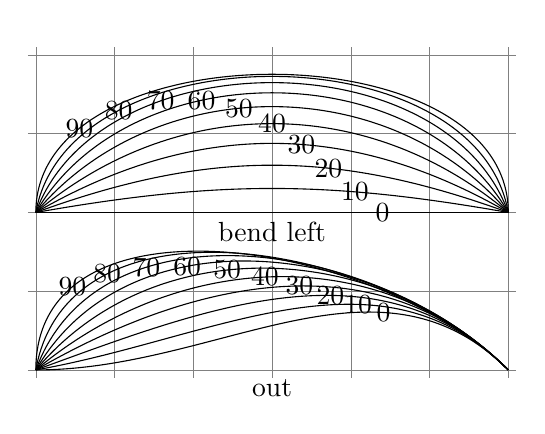
\begin{tikzpicture}
\draw[help lines] (-0.1,-0.1) grid (6.1,4.1);

\foreach \i in {0,10,...,90}{
    \draw (0,2) to[bend left=\i]node[pos=.75-\i/160]{\i} +(6,0);
}
\node[below] at (3,2){bend left};

\foreach \i in {0,10,...,90}{
    \draw (0,0) to[out=\i]node[pos=.7-\i/180]{\i} +(6,0);
}
\node[below] at (3,0){out};

\end{tikzpicture}
\end{document}
